
\documentclass[UTF8,12pt]{ctexart}



%二、字体
    %\setmainfont{fontName}  %英文的
    %\setsansfont{fontName}  %去设置-字体找fontName
    %\setmonofont{fontName}
    \setCJKmainfont{宋体}   %设置主字体族
    \setCJKsansfont{黑体}   %设置无衬线字体族
    \setCJKmonofont{楷体}   %设置打字机字体族
    %\textrm{}和\rmfamily, \textsf{}和\sffamily, \texttt{}和\ttfamily 
    %可以让我们分别主动调用主字体族,无衬线字体族和打字机字体族 

    %可以使用\textup{}和\upshape, \textit{}和\itshape
    %来分别主动调用当前字体族的直立体与意大利斜体

    %用\textmd{}和\mdseries, \textbf{}和\bfseries
    %来分别调用当前字体形状的正常体与粗体。



%字号:https://blog.csdn.net/c_arm/article/details/7013462



%五、行距与缩进
    \usepackage{setspace}  %行距
    \setstretch{1.2}       %填比例
    \setlength{\parskip}{1em}  %设置额外的段间距
    %  当前的字体大小被记作单位em, 也就是说,如果当前字号为12pt, 那当前1em=12pt.
    %  \setlength{\parindent}{2em}  设置缩进距离为2em
    %  \setlength{\parindent}{0em}  取消缩进



%六、附录与文献
    \newcommand{\upcite}[1]{\textsuperscript{\cite{#1}}} 
    %这使得我们可以在正文调用将编号置于右上角的参考文献

    \usepackage[toc, page]{appendix} 
    \renewcommand{\appendixtocname}{附录}
    \renewcommand{\appendixpagename}{附录}
    %这使得我们可以写附录



%七、列表
    \usepackage{enumitem}  %用于自定义列表

    %1. 定义问题一,问题二...列表,用question调用
        \newlist{question}{enumerate}{1}
        \setlist[question,1]{itemsep = 0pt, parsep = 0pt, align=left, leftmargin=*, label = {\bfseries 问题\chinese*}}

    %2. 定义问题一,问题二...列表,用zombie调用
        \newlist{zombie}{enumerate}{1}
        \setlist[zombie,1]{itemsep = 0pt, parsep = 0pt, align=left, leftmargin=*, label = {\bfseries 僵尸\chinese*}} 

    %\renewcommand{\theenumi}{\chinese{enumi}}
    %可以使第一级编号时出现的不是1 2 3而是一二三

    %\renewcommand{\labelenumi}{(\theenumi)}
    %可以使1.2.3.变成(1)(2)(3)

    %\renewcommand{\labelitemi}{随便符号}
    %可以改变无序列表的模样。比如填入空心圆圈$\circ$,或者更夸张填$\sum$等等



%八、纸张与页面
    \usepackage{fancyhdr}     %页面设置包
    \pagestyle{fancy}         
    \fancyhf{}
    \usepackage{geometry}  

    %1.页面与版心
        %(1)使用A4纸:               
        \geometry{a4paper}
        %(2)以数值形式指定纸张大小:   \geometry{paperheight=22cm, paperwidth=10cm}
        %(3)边距设置:边距有上下左右————left, right, top, bottom
            %\geometry{left=2cm}    %设置左边距为2cm
            %\geometry{right=2cm}
            %\geometry{top=2cm}
            %\geometry{bottom=2cm}
        %(4)版心水平居中:\geometry{hcentering}      版心竖直居中:\geometry{vcentering} 
        \geometry{hcentering}
        %(5)版心长设置:\geometry{textheight=20cm}   版心宽设置:\geometry{textwidth=20cm}

    %2.页眉与页脚    (先加载fancyhdr包)
        %(1)页眉页脚的左中右共6部分对应代码:
            %\lhead{}, \chead{}, \rhead{}, \lfoot{}, \cfoot{}, \rfoot{}
            \chead{“深圳杯”数学建模挑战赛}   
            \rhead{\thepage}
            %\chead{学习指南}  %在页眉正中出现“学习指南” 
        %(2)页眉线与页脚线:  \headrulewidth和\footrulewidth
            %\renewcommand\headrulewidth{0pt}   输入参数决定粗细,0则取消该线
            \renewcommand\headrulewidth{0pt}



%九、图片
    \usepackage{graphicx}           %四个包
    \usepackage{float}
    \usepackage{caption}
    \usepackage[export]{adjustbox}  %解决过宽图片

    %1.
    %\captionsetup[figure]{name=图片,font={Large, it}}   
    %将图片描述 “图X: ” 改成 “图片X: ”
    %将序号改为"it":意大利斜体,全部字体改成\Large
     
    %2.
    \captionsetup[figure]{name=图片} 
    %将图片描述设置为 “图片X: ”(默认)
    %texdoc caption 查看文档得到所有font,上面的it就是一种



%十、表格
    \usepackage{float}         %基础包
    \usepackage{booktabs}      %Excel2LaTeX美观选项支持
    \usepackage{longtable}     %过长表格
    %\usepackage{adjustbox}    %过宽表格包,但有另外的方法

    %1.
    \captionsetup[table]{font=large}
    %把“表 1”字体调大,格式类似九、2.



%十一、图片与表格的编号
    %\counterwithin{table}{section}    %让表格在section内编号
    %\counterwithin{figure}{section}   %让图片在section内编号
    %交叉引用!!!!:          使用\label \ref  均需要编译两次



%十二、数学
    \usepackage{amsmath}         %基础包
    \usepackage{esint}           %积分号美观包
    \usepackage{unicode-math}    %数学环境字体宏包

    %1.定义dx中d的立直体。用'\dif x'来输入正规的'dx'
    \def\dif{\mathop{}\!{}\mathrm{d}}



    \usepackage{caption} 



\begin{document}



\begin{titlepage}  %封面
    \centering
    \vspace*{\stretch{0}}{
        \huge{
            \textrm{
                2019\textbf{年“深圳杯”数学建模挑战赛}\\
                \ \\
                B\textbf{题}\\
                \ \\
                \ \\
                \ \\
                \textbf{新一代通信网络设计与规划}
            }
        }
    }\\

    \vspace{\stretch{2}}{
        \ \\
        \ \\
        \ \\
        \ \\
        \ \\
        \begin{align*}
            \text{\zihao{-2}中山大学:}\ \ &\text{\zihao{-2}林天皓}\\
            &\text{\zihao{-2}龙行健}\\
            &\text{\zihao{-2}卢浩文}
        \end{align*}
        }\\

    \vspace{\stretch{3}}
    {\today}
\end{titlepage}
    



%二、目录
\tableofcontents



%三、正文
\section{摘要}




\section{问题重述与分析}
    \subsection{微波问题1}分析题目可知,
        我们的相控阵天线由32个天线组成,每一个天线能发出相对独立的波束,
        这些波束之间互相叠加与干涉,
        最终我们的相控天线<各个波束信号之间是如何叠加与干涉的模型>,
        然后对这32根各有5种移相器配置方式(包括关闭波束)的天线找到一种
        波束配置方式,使得叠加这些波束,发出的信号在水平角$AZ = 10°$,
        俯仰角$EL= 5°$的方向上合成功率大于$35dBm$,同时为了避免对在位置$AZ=10°$,
        俯仰$EL=10°$站点的干扰,需要发出的信号在水平角$AZ=10°$,
        俯仰角$EL=10°$的方向上的合成功率尽可能小,为了避免减小旁瓣,
        还要求其他方向的合成功率尽可能小。我们对这三个目标进行了量化分析,
        建立了<波束配置方式效用评价模型>。由于配置方式种类多达$5^{32}$种,
        传统的遍历式搜索无法在有限时间内给出一个最优解,
        而遗传算法非常善于解决这种搜索空间庞大,目标明确的问题,
        所以我们选择使用遗传算法求解。

    \subsection{微波问题2}
        与上题不同的是,该题不是要求单个方向的合成功率达到$35dBm$,
        而是在共有$91$个方向的一片区域上的平均功率达到$35dBm$,
        其次为了保证接收机在这片区域上的信号强度相对稳定,
        凹坑尽可能小——即在这片区域上信号功率的极差尽可能小,
        同时关闭尽可能多的天线加快扫描速度。针对这三个目标,我们需要对这些问题量化,
        同时建立<区域覆盖评价模型>,鉴于该问题的搜索空间与微波问题一相同,
        我们继承了问题一采用的遗传算法搜索一种使得评价函数值尽可能大的配置方式。

     
    \subsection{骨干网问题1}
    \subsection{骨干网问题2}
        对于骨干网问题二,可以不需要满足整个网络的需求,
        要取得效益最大的网络建设效果。不难估计,
        建设骨干网络是一个边际效益递减的工程,
        覆盖最后百分之十的成本一定比覆盖前百分之十的成本要高,
        所以我们设定骨干网络建设效率函数评估当前选定的网络建设方式,成本尽可能低,
        覆盖率(当前网络建设下满足的流量/全省流量)尽可能大。对于这个二元函数,
        我们逐个参数考虑,先考虑覆盖率一定时候成本最低是多少,
        接下来找到性价比(覆盖率/成本)最高的点,得到接入网络价值最大的部署方案。
        
        



\section{模型假设}\label{mxjs}
    \subsection{微波问题}
        \begin{enumerate}
            \item 假设微波接收机在无穷远处,即微波接收机与所有阵列天线的角度相等
            \item 在所给的测量数据中,相控天线每$5°$给出一组实际测量数据,我们以其数据
                代表其附近$2.5°$区域内的信号强度和相位。
            \item 功率与相位实际测量数据中的空数据($inf$和$nan$数据)均视为0进行处理
        \end{enumerate}
    

    \subsection{骨干网问题}
        \begin{enumerate}
            \item 各个城市、人群的实际数据需求量总体随时间递增,但它并不是随时间一直增加的——
                例如,每一天,用户带宽需求都会随着时辰的改变而改变。
                信息网络的部署实际上应该着眼于每天/每周的用网高峰期。
                则在本文中,我们讨论的“数据需求量”均表示每天/每周用网高峰期的实际数据需求量。

            \item 骨干网承担各城市对外网络交互的出入口功能,起止点应该设于各个城市中心
                我们合理地假设所有光缆铺设的起止点位于各个城市的市政府附近,并以各市市政府
                位置为标准测量各城市间的距离。
            
            \item 光缆的铺设与维护是一项专业性工作,不需要像铺设公路考虑驾驶员安全一样苛刻。
                在铺设光缆时,只需要避开极端地形。不考虑海拔变化/地形因素对光缆长度的影响,
                我们合理地假设在两城间铺设光缆时,成本最低的方案大致为全线沿直线铺设。依此,
                一并假设光缆的成本仅由起止点、线路类型、光缆中光纤数目决定。

            \item 不考虑光缆的铺设时间。
            \item 假设未来用户数据需求量呈指数形式的增长。
            \item 假设广东省各城市未来十年人口基本不变。
            \item 由于潮汕三市——汕头、揭阳、潮州所选基点(市政府)距离极小,且基本可以确定
                最佳连接方案就是广州-……-揭阳,揭阳-汕头,揭阳-潮州。则在构建蚁群算法模型和
                最小生成树模型时,将潮汕三市作为一个整体考虑
        \end{enumerate}





\section{符号说明}
    \subsection{微波问题}
        \begin{enumerate}
            \item $k$ :单天线的五种配置方式,取值为$0,1,2,3,4$,
            分别代表该天线:关闭$,$位移$0°,90°,180°,270°$
            \item $\overrightarrow{e_i}$ :单个天线在区域中某点产生的信号矢量
            \item $w_i$ :单个天线在区域中某点产生的功率强度
            \item $\overrightarrow{E_i}$ :32个天线在区域内某点叠加后的矢量
            \item $|\overrightarrow{E_i}|$ :32个天线在区域内某点叠加后的矢量强度
            \item $\varphi_{ik}$ :单个天线在区域内某点的配置方式下相位大小,k在此处不等于0
            \item $G_v$ :目标点功率值
            \item $I_v$ :干扰点功率值
            \item $O_v$ :单个个体的适应值
            \item $W = 20\cdot log_{10}{|\overrightarrow{E}|}$:功率和信号强度的转化公式
        
       
        \end{enumerate}
    
    \subsection{骨干网问题}
      \subsubsection{数据需求模型}
        \begin{enumerate}
            \item $O$层:数据需求的层次结构中的目标层,即数据需求量。
            \item $C$层:数据需求的层次结构中的准则层,包括了商业需求、个人需求、行政需求。
            \item $D$层:数据需求的层次结构中的决定层,包括了年龄、收入、人口。
            \item $A_{X-Y}$:$X$层的所有元素对上一层$Y$元素之影响的成对比较矩阵
            \item $\lambda _{max}$:
                成对比较矩阵的最大特征值(或其组成的向量)
            \item $\overrightarrow\omega _{C-O}$:
                $A_{C-O}$的最大特征值所对应的特征向量,称为权向量
            \item $W_{D-C}$:$A_{D-C_1},A_{D-C_2},A_{D-C_3}$的最大
                特征值分别对应的特征向量组成的矩阵,称为权向量矩阵
            \item $n_{x-y}$:进行成对比较的元素数目
            \item $CI_{X-Y}$:层次分析中的一致性指标
            \item $RI_{X-Y}$:层次分析中的平均随机一致性指标
            \item $CR_{X-Y}$:层次分析中的随机一致性比率
        \end{enumerate}
      
      \subsubsection{城市评分模型}
        \begin{enumerate}
            \item $C_k$:城市k
            \item $Y_k$:城市k的平均年龄
            \item $x_{k1}$:城市k的年龄得分
            \item $I_k$:城市k的人均可支配收入
            \item $x_{k2}$:城市k的收入得分
            \item $P_k$:城市k的人口
            \item $x_{k3}$:城市k的人口得分
            \item $x_k$:城市k的(加权后)总得分
            \item $N_k$:城市k的数据需求量
        \end{enumerate}

      \subsubsection{蚁群算法模型}
        \begin{enumerate}
            \item $n$:城市数量
            \item $d_{k_1k_2}$:城市$k_1,k_2$的距离
            \item $N_k$:城市k的数据需求量
            \item $N_{k_1k_2}$:城市$k_1,k_2$的数据需求量之和
            \item $a$:蚁群算法信息素权重参数
            \item $b$:蚁群算法原始权重参数
            \item $c$:蚁群算法信息素挥发速度参数
            \item $d$:蚂蚁走过路线时该线路增加的信息素含量
            \item $s$:蚂蚁种群数量
            \item $P_i$:蚂蚁向其他城市移动的概率向量
            \item $T_{ij}$:城市$k_1,k_2$之间路线的信息素含量
        \end{enumerate}





\section{模型建立}
    \subsection{微波相关1.2.3.4.5}


    \subsection{数据需求模型}\label{ShuJv}
            \begin{figure}[]
                    \centering
                    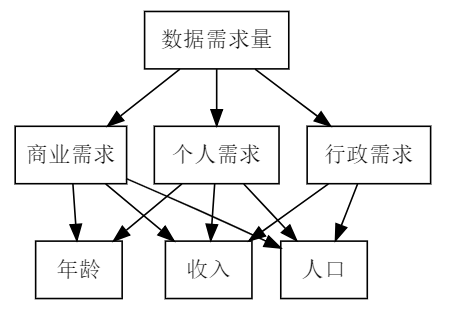
\includegraphics{need.png}
                    \caption{数据需求层次结构}\label{SJXQCCJG}
                \end{figure}
        建立层次结构模型,如图片\ref{SJXQCCJG},这个图会乱跑最终定稿再来调浮动体参数固定他。

        \begin{enumerate}
            \item C层对数据需求量的影响:
            \begin{enumerate}
                \item 建立成对比较矩阵:
                $A_{C-O}=\begin{bmatrix}
                    1 & \frac{1}{4} & 4 \\                    
                    4 & 1 & 8\\                  
                    \frac{1}{4} & \frac{1}{8} & 1
                 \end{bmatrix}$
                \item 求得最大特征值$\lambda _{max}=3.0536$及其对应的权向量为
                    $$\overrightarrow\omega_{C-O}=(0.2227,0.7071,0.0702)$$
                \item 由$n_{c-o}=3$,求得$A_{C-O}$的一致性指标$CI_{C-O}=0.0268$
                \item 由$n_{c-o}=3$,得平均随机一致性指标$RI_{C-O}=0.58$,
                    则随机一致性比率$CR_{C-O}=0.0462<0.1$,接受该层分析。\\
            \end{enumerate}
            则认为商业需求,个人需求,行政需求对数据需求量影响的比重分别为$0.2227,0.7071,0.0702$。
              
            \item D层对数据需求量的影响:
            \begin{enumerate}
                \item 为D层对商业需求的影响建立成对比较矩阵:
                $$A_{D-C_1}=\begin{bmatrix}
                    1 & \frac{1}{8} & \frac{1}{6} \\
                    8 & 1 & 1\\
                    6 & 1 & 1
                 \end{bmatrix}$$
                \item 为D层对个人需求的影响建立成对比较矩阵:
                $$A_{D-C_2}=\begin{bmatrix}
                    1 & \frac{1}{2} & \frac{1}{8} \\
                    2 & 1 & \frac{1}{7}\\
                    8 & 7 & 1
                 \end{bmatrix}$$
                \item 为D层对行政需求的影响建立成对比较矩阵:\\(其中$D_1$不影响行政需求)
                $$A_{D-C_3}=\begin{bmatrix}
                    1 & \frac{1}{2}\\
                    2 & 1
                 \end{bmatrix}$$
                \item \begin{itemize}
                    \item 求得这三个成对比较矩阵的最大特征值向量为$$\lambda _{max}=(3.0092,3.0349,2)$$
                    \item 其对应的权向量矩阵为$$W_{D-C}=\begin{bmatrix}
                        0.0672 & 0.0813 & 0 \\
                        0.4887 & 0.1349 & 0.3333 \\
                        0.444  & 0.7838 & 0.6667
                     \end{bmatrix}$$
                    \item 对应的D层对O层的组合权向量为$$\omega_{D-O}=\begin{bmatrix}
                        0.0672 & 0.0813 & 0 \\
                        0.4887 & 0.1349 & 0.3333 \\
                        0.444  & 0.7838 & 0.6667
                     \end{bmatrix}×\begin{bmatrix}
                        0.2227 \\
                        0.7071 \\
                        0.0702
                     \end{bmatrix}=\begin{bmatrix}
                        0.0725 \\
                        0.2276 \\
                        0.6999
                     \end{bmatrix}$$
                    \end{itemize}                    
                \item 则D层对C层的一致性指标为
                    $$CI_{D-C}=[0.0046,0.0174,0]×\begin{bmatrix}
                    0.2227 \\
                    0.7071 \\
                    0.0702
                     \end{bmatrix}=0.0133$$
                \item 又有D层对C层的平均随机一致性指标为
                    $$RI_{D-C}=[0.58,0.58,0]×\begin{bmatrix}
                    0.2227 \\
                    0.7071 \\
                    0.0702
                     \end{bmatrix}=0.5393$$
                \item 则D层对O层的组合随机一致性比率为
                    $CR_{D-O}=0.0462+\displaystyle\frac{0.0133}{0.5393}=
                    0.0709<0.1$,接受该层分析。
            \end{enumerate}

        \end{enumerate}
        综上,得到年龄,收入,人口对数据需求量影响的比重分别为$0.0725,0.2276,0.6999$
        


    \subsection{城市评分模型}\label{PingFen}
        \subsubsection{平均年龄评分}
            当今社会中的年轻人,特别是大学生使用互联网教多,数据需求量较大。
            数据需求量的峰值大约在年龄为15岁~25岁之间达到。
            广东省内各城市平均年龄均大于30岁,则年龄与数据需求量大致可视为负相关,
            则选择以反比例尺度对平均年龄评分
            \begin{itemize}
                \item 以广州市的平均年龄$Y_1=34.4$岁为100分
                \item 某市$C_k$的平均年龄为$Y_k$,满足$Y_1=\displaystyle\frac{x_{k1}}{100}·Y_k$,则该市年龄得分为$x_{k1}$
                \item 任一城市$C_k$的年龄得分为$$x_{k1}=\frac{100Y_1}{Y_k}$$
            \end{itemize}

        \subsubsection{人均可支配收入评分}
            数据需求量应当与收入呈正相关,但随着收入的增加,
            数据需求量的增长率不会一直保持水平,应该随收入的增加而逐渐降低。
            则选择以对数尺度对人均可支配收入评分:
            \begin{itemize}
                \item 以广州市人均可支配收入为100分\par 
                    (\ 设广州市人均可支配收入$I_1=5.5356=a^{100}$万元\ )
                \item 某市$C_k$的人均可支配收入$I_k=a^{x_{k2}}$万元,则该市收入得分为$x_{k2}$
                \item 任一城市$C_k$的收入得分为$$x_{k2}=\log _{I_1}({I_k}^{100})=\frac{100\ln I_k}{\ln I_1}$$
            \end{itemize}

        \subsubsection{人口评分}
            由于城市需求量大致是每个群体的群体需求量的总和,
            所以人口与数据需求量大致成线性关系。则选择以线性尺度对城市人口评分
            \begin{itemize}
                \item 以广州市的人口$P_1=1490.44$万人为100分
                \item 某市$C_k$的人口为$P_k$,
                    则该市的人口得分为$$x_{k3}=\frac{100P_k}{P_1}$$
            \end{itemize}
    
    \subsection{蚁群算法模型}\label{YQSFMX}
        \begin{enumerate}
            \item 根据每两个城市之间的距离$d_{ij}$和
            每两个城市数据需求量之和$N_{ij}=N_i+N_j$,建立路径的原始权重邻接矩阵
            $$D_{ij}=\frac{N_{ij}}{d_{ij}}$$
            \item 创建信息素邻接矩阵$T$,大小与$D$相同
            \item 对$s$只每只蚂蚁随机选取城市$i$做为起点
            \item 对于每只蚂蚁,计算蚂蚁向其他城市移动的概率向量$P_i$
            $$P_i=\left[\frac{D_{i1}^bT_{i1}^a}{\sum_{k=1}^n{D_{ik}^bT_{ik}^a}}~\frac{D_{i2}^bT_{i2}^a}{\sum_{k=1}^n{D_{ik}^bT_{ik}^a}}~··· \frac{D_{in}^bT_{in}^a}{\sum_{k=1}^n{D_{ik}^bT_{ik}^a}}\right]$$
            \item 蚂蚁按照概率$P_i$选择移动的路线,
                选择向j点移动把该条线路上的信息素含量$T_{ij}$增加$d$,
                若蚂蚁的位置已经在广州,则不再使得该蚂蚁移动
            \item 信息素挥发,令$T=(1-c)T$
            \item 循环步骤3到步骤5多次,最终每只蚂蚁都到达广州,算法终止,
            得到最终的信息素矩阵$T$,
            分析信息素矩阵中信息素含量较大的路线为相对重要的路线
        \end{enumerate}

    \subsection{最小生成树模型}\label{ZXSCSMX}
 




\section{问题求解}
    \subsection{微波问题1}
    \subsection{微波问题2}
    \subsection{骨干网问题1}
        \subsubsection[网络需求评估]{各城市数据需求量评估}\label{WLXQPG}
            对广东省各城市人口、平均年龄、人均可支配收入\upcite{CSSJ},
            根据\ref{PingFen}城市评分模型进行评分,
            并根据\ref{ShuJv}数据需求模型评价各个城市的需求总分。
            以xxxxxxx为标准,得到单位分数对应的数据需求量,
            以此评估广东省各城市的数据需求量。

        \subsubsection[网络部署方案]{网络部署方案的设计}    
            借助\ref{WLXQPG}中获取的各城市数据需求量:
            \begin{enumerate}
                \item 使用\ref{YQSFMX}:蚁群算法模型,选取的参数为
                    \begin{itemize}
                        \item $n=19$ (客观事实,其中广州市编号为1)
                        \item $a=2$
                        \item $b=1$ (蚁群算法原始权重参数)
                        \item $c=0.3$ (蚁群算法信息素挥发速度参数)
                        \item $d=0.3$蚂蚁走过路线时该线路增加的信息素含量
                        \item $s=50$蚂蚁种群数量最终将信息素含量的大小作为边的粗细
                    \end{itemize}
                得到:
                    \begin{figure}[H]
                      \centering
                      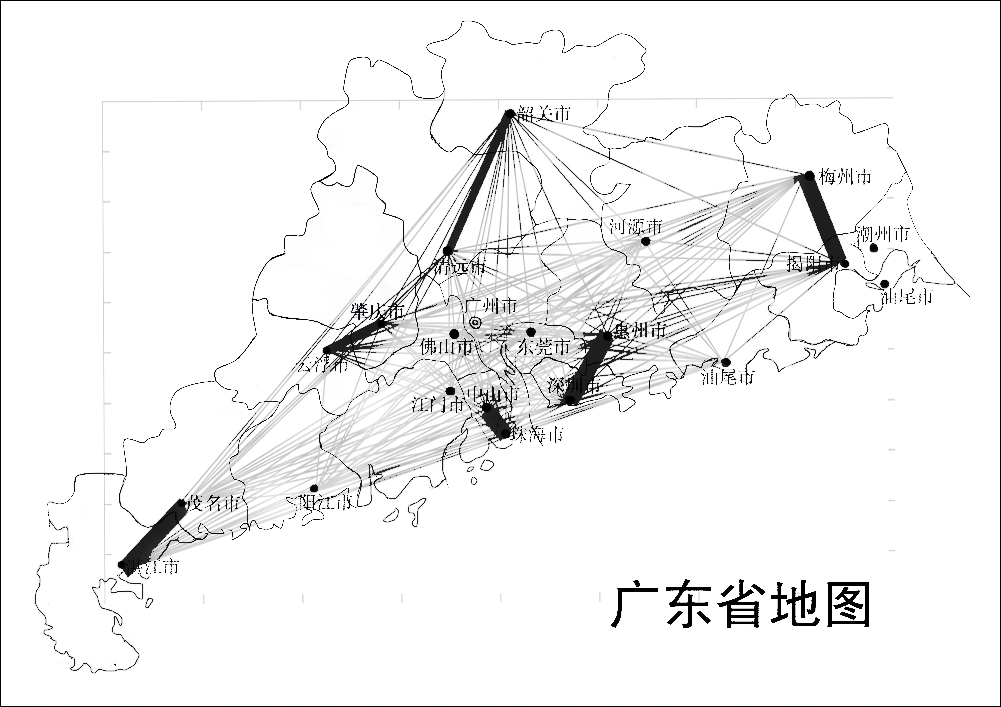
\includegraphics[scale=0.32]{YQSF.png}   %输入文件绝对路径。如果同文件夹下就不用
                      \caption{蚁群算法方案}
                      \end{figure}
                我们决定以这些边为基础创建网络
                \item 使用\ref{ZXSCSMX}:最小生成树模型,得到:
                    \begin{figure}[H]
                      \centering
                      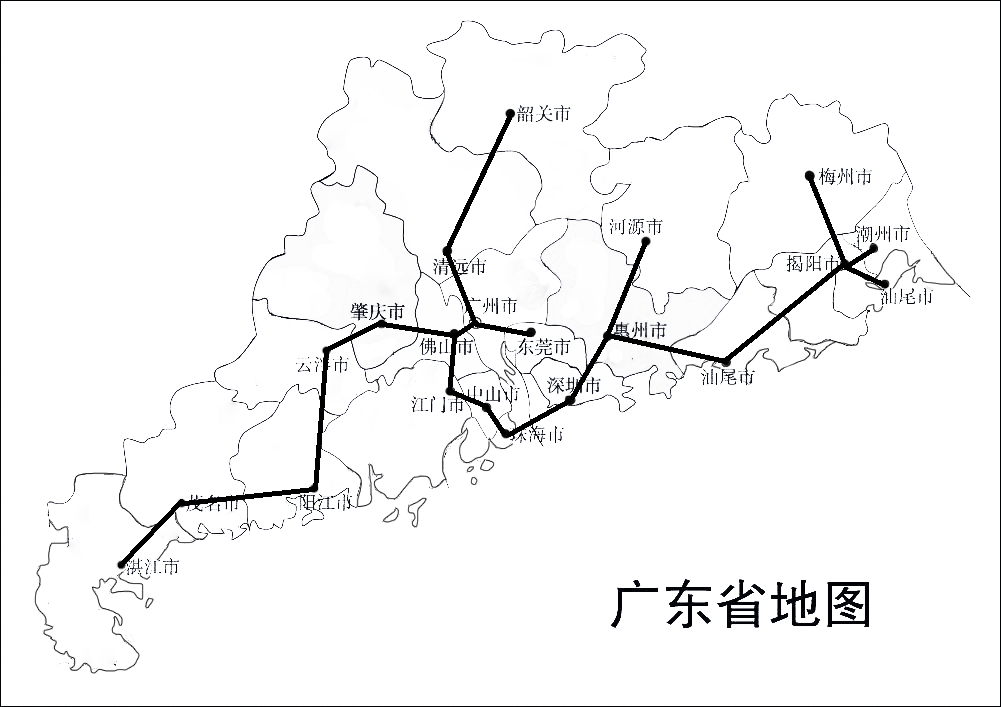
\includegraphics[scale=0.6]{ZXSCS.png}   %输入文件绝对路径。如果同文件夹下就不用
                      \caption{最小生成树方案}
                      \end{figure} 
            \end{enumerate}

            可以发现最小生成树算法得到的线路网络与蚁群算法的结果非常吻合,
            综合两个模型考虑,我们剔除了珠海到深圳横跨珠江的不符合现实的线路,
            在江门到佛山,肇庆到清远,深圳到惠州之间加入了网络线路,
            期望平衡网络流量的负载。最终确定了部署方案:
            \begin{figure}[H]
                \centering
                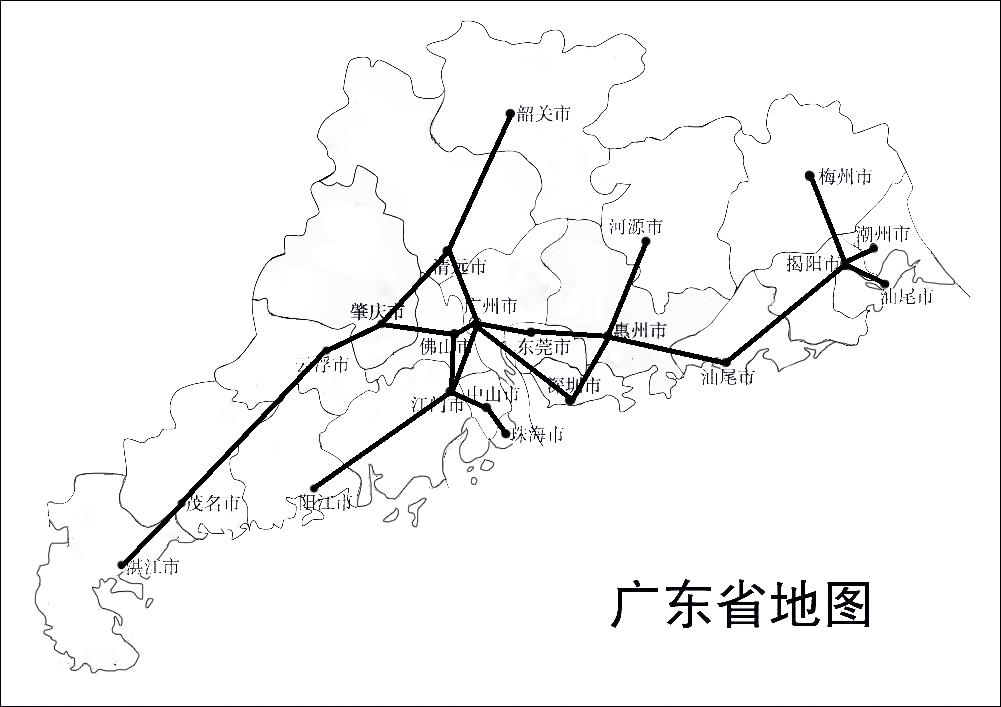
\includegraphics[scale=0.7]{over.png}   %输入文件绝对路径。如果同文件夹下就不用
                \caption{网络部署方案}
                \end{figure}

    \subsection{骨干网问题2}

    \newpage
\section{还需要整理排版}
    \begin{enumerate}
        \item 问题分析lthmd中的骨干网问题1(等lth把最后一句的逻辑处理完)
        \item 微波问题论文 md中除符号外全部(两个模型,两个求解)
        \item \ref{WLXQPG}中的xxx标准(回归分析)
        \item 所有代码
    \end{enumerate}
\section{还需要撰写初稿}
    \begin{enumerate}
        \item 最小生成树模型解析
        \item 微波问题论文 md中除符号外全部
    \end{enumerate}
        \newpage




%五、文献
\begin{thebibliography}{20}   %表示参考文献最大数量
    %每个bibitem表示一份文献
    %第一个参数这里没用(不显示),用于交叉引用
    %第二个参数就是显示的内容
    \bibitem{CSSJ}{广东省统计局,广东统计信息网(及首页中各市链接), \\
        http://stats.gd.gov.cn/, 2019.5.12.}
    \bibitem{yjJJ}{中华人民共和国工业和信息化部,2019年1-4月份通信业经济运行情况,\\
        http://www.miit.gov.cn/n1146285/n1146352/n3054355/n3057511/\\
        n3057518/c6969297/content.html,2019.5.31}
    \bibitem{yqJJ}{中华人民共和国工业和信息化部,2017年1-4月份通信业经济运行情况,\\
        http://www.miit.gov.cn/n1146312/n1146904/n1648372/c5653421/\\
        content.html,2019.5.31}
    \bibitem{ylJJ}{中华人民共和国工业和信息化部,2016年8月份通信业经济运行情况,\\
        http://www.miit.gov.cn/n1146285/n1146352/n3054355/n3057511/\\
        n3057518/c5264001/content.html,2019.5.31}
    \bibitem{ywJJ}{中华人民共和国工业和信息化部,2015年7月份通信业经济运行情况,\\
        http://www.miit.gov.cn/n1146285/n1146352/n3054355/n3057511/\\
        n3057518/c3602990/content.html,2019.5.31}
    \bibitem{ysJJ}{中华人民共和国工业和信息化部,2014年6月份通信业经济运行情况,\\
        http://www.miit.gov.cn/n1146312/n1146904/n1648372/c3336719/\\
        content.html,2019.5.31}
    
    %文献按正文中的引用次序列出,其中书籍的表述方式为:
    %[编号] 作者,书名,出版地:出版社,出版年。
    %参考文献中期刊杂志论文的表述方式为:
    %[编号] 作者,论文名,杂志名,卷期号:起止页码,出版年。
    %参考文献中网上资源的表述方式为:
    %[编号] 作者,资源标题,网址,访问时间(年月日)。
\end{thebibliography}



%四、附录
\begin{appendices}
    \section{数据需求量评估}\label{fuluCSSJ}
      \begin{table}[H]
        \centering
        \caption*{\small{(数据来自\cite{CSSJ})}}
          \begin{tabular}{cccccccccc}
          \toprule
          1      & $C_k$ & $Y_k$ & $x_{k1}$ & $I_k$ & $x_{k2}$ & $P_k$ & $x_{k3}$ & $x_k$ & $N_k$ \\
          \midrule
          2      & 广州     & 34.4   & 100    & 5.54   & 100    & 1490.4 & 100    & 100    & 15.24 \\
          \midrule
          3      & 佛山     & 34.4   & 100    & 4.96   & 93.62  & 790.57 & 53.04  & 65.68  & 10.01 \\
          \midrule
          4      & 东莞     & 30.6   & 112.4  & 4.93   & 93.27  & 839.22 & 56.31  & 68.79  & 10.48 \\
          \midrule
          5      & 江门     & 34.5   & 99.71  & 2.95   & 63.31  & 459.82 & 30.85  & 43.23  & 6.588 \\
          \midrule
          6      & 清远     & 34.5   & 99.71  & 2.24   & 47.05  & 387.4  & 25.99  & 36.13  & 5.505 \\
          \midrule
          7      & 中山     & 33.5   & 102.7  & 4.69   & 90.27  & 331    & 22.21  & 43.53  & 6.634 \\
          \midrule
          8      & 肇庆     & 31.7   & 108.5  & 2.41   & 51.33  & 415.17 & 27.86  & 39.05  & 5.95 \\
          \midrule
          9      & 珠海     & 33.4   & 103    & 4.81   & 91.8   & 189.11 & 12.69  & 37.24  & 5.675 \\
          \midrule
          10     & 深圳     & 32.1   & 107.2  & 5.75   & 102.3  & 1302.7 & 87.4   & 92.22  & 14.05 \\
          \midrule
          11     & 惠州     & 31.6   & 108.9  & 3.39   & 71.4   & 483    & 32.41  & 46.82  & 7.135 \\
          \midrule
          12     & 云浮     & 31.2   & 110.2  & 1.92   & 38.24  & 252.69 & 16.95  & 28.56  & 4.352 \\
          \midrule
          13     & 韶关     & 34.7   & 99.14  & 2.37   & 50.37  & 299.76 & 20.11  & 32.73  & 4.987 \\
          \midrule
          14     & 河源     & 31.7   & 108.5  & 1.94   & 38.72  & 309.39 & 20.76  & 31.21  & 4.756 \\
          \midrule
          15     & 阳江     & 32.9   & 104.6  & 2.32   & 49.05  & 255.56 & 17.15  & 30.75  & 4.685 \\
          \midrule
          16     & 湛江     & 32.5   & 105.8  & 2.14   & 44.53  & 733.2  & 49.19  & 52.24  & 7.96 \\
          \midrule
          17     & 茂名     & 30.9   & 111.3  & 2.14   & 44.32  & 631.32 & 42.36  & 47.81  & 7.285 \\
          \midrule
          18     & 汕尾     & 31.3   & 109.9  & 2.1    & 43.36  & 299.36 & 20.09  & 31.89  & 4.86 \\
          \midrule
          19     & 揭阳     & 32     & 107.5  & 2      & 40.63  & 608.94 & 40.86  & 45.64  & 6.954 \\
          \midrule
          20     & 汕头     & 32.5   & 105.8  & 2.44   & 52.19  & 563.85 & 37.83  & 46.03  & 7.014 \\
          \midrule
          21     & 潮州     & 34.3   & 100.3  & 2.09   & 43.09  & 265.66 & 17.82  & 29.55  & 4.504 \\
          \midrule
          22     & 梅州     & 33.8   & 101.8  & 2.12   & 43.96  & 437.88 & 29.38  & 37.95  & 5.782 \\
          \midrule
                 & 总和     &        & 2207   &        & 1293   &        & 761.3  & 987    & 150.4 \\
          \bottomrule
          \end{tabular}%
      \end{table}%

    

    
    \section{遗传算法模型——微波问题一 Matlab代码}
    \section{遗传算法模型——微波问题二 Matlab代码}
    \section{蚁群算法模型Matlab代码}
    \section{最小生成树算法模型Matlab代码}
\end{appendices} 

\end{document}         